This chapter describes the specific implementation details of the IDDR and its communication channel.

\section{Implementation Overview} 
The IDDR system is implemented with Linux kernel 3.5.0 and Xen hypervisor 4.2.1. For the prototype, we implemented the IDDR system with the isolated block device driver. Both the application domain and the driver domain run the same Linux kernel. The following table summarizes our implementation efforts of the IDDR system. 

\begin{center}
\begin{tabular}{|r|l|} 
  \hline
  Component & Number of Lines \\
  \hline
  Linux Kernel & 7 \\
  Xen & 250 \\
  Front-end Driver & 647 \\
  Back-end Driver & 752 \\
  \hline 
  Total & 1656\\
  \hline
\end{tabular}
\end{center}

As we observe from the table, the block device driver is unchanged, small number of changes were made to the Linux kernel and the Xen hypervisor. However, we maintain the application compatibility.

\section{Implementation}

\begin{figure}[!ht]
\centering
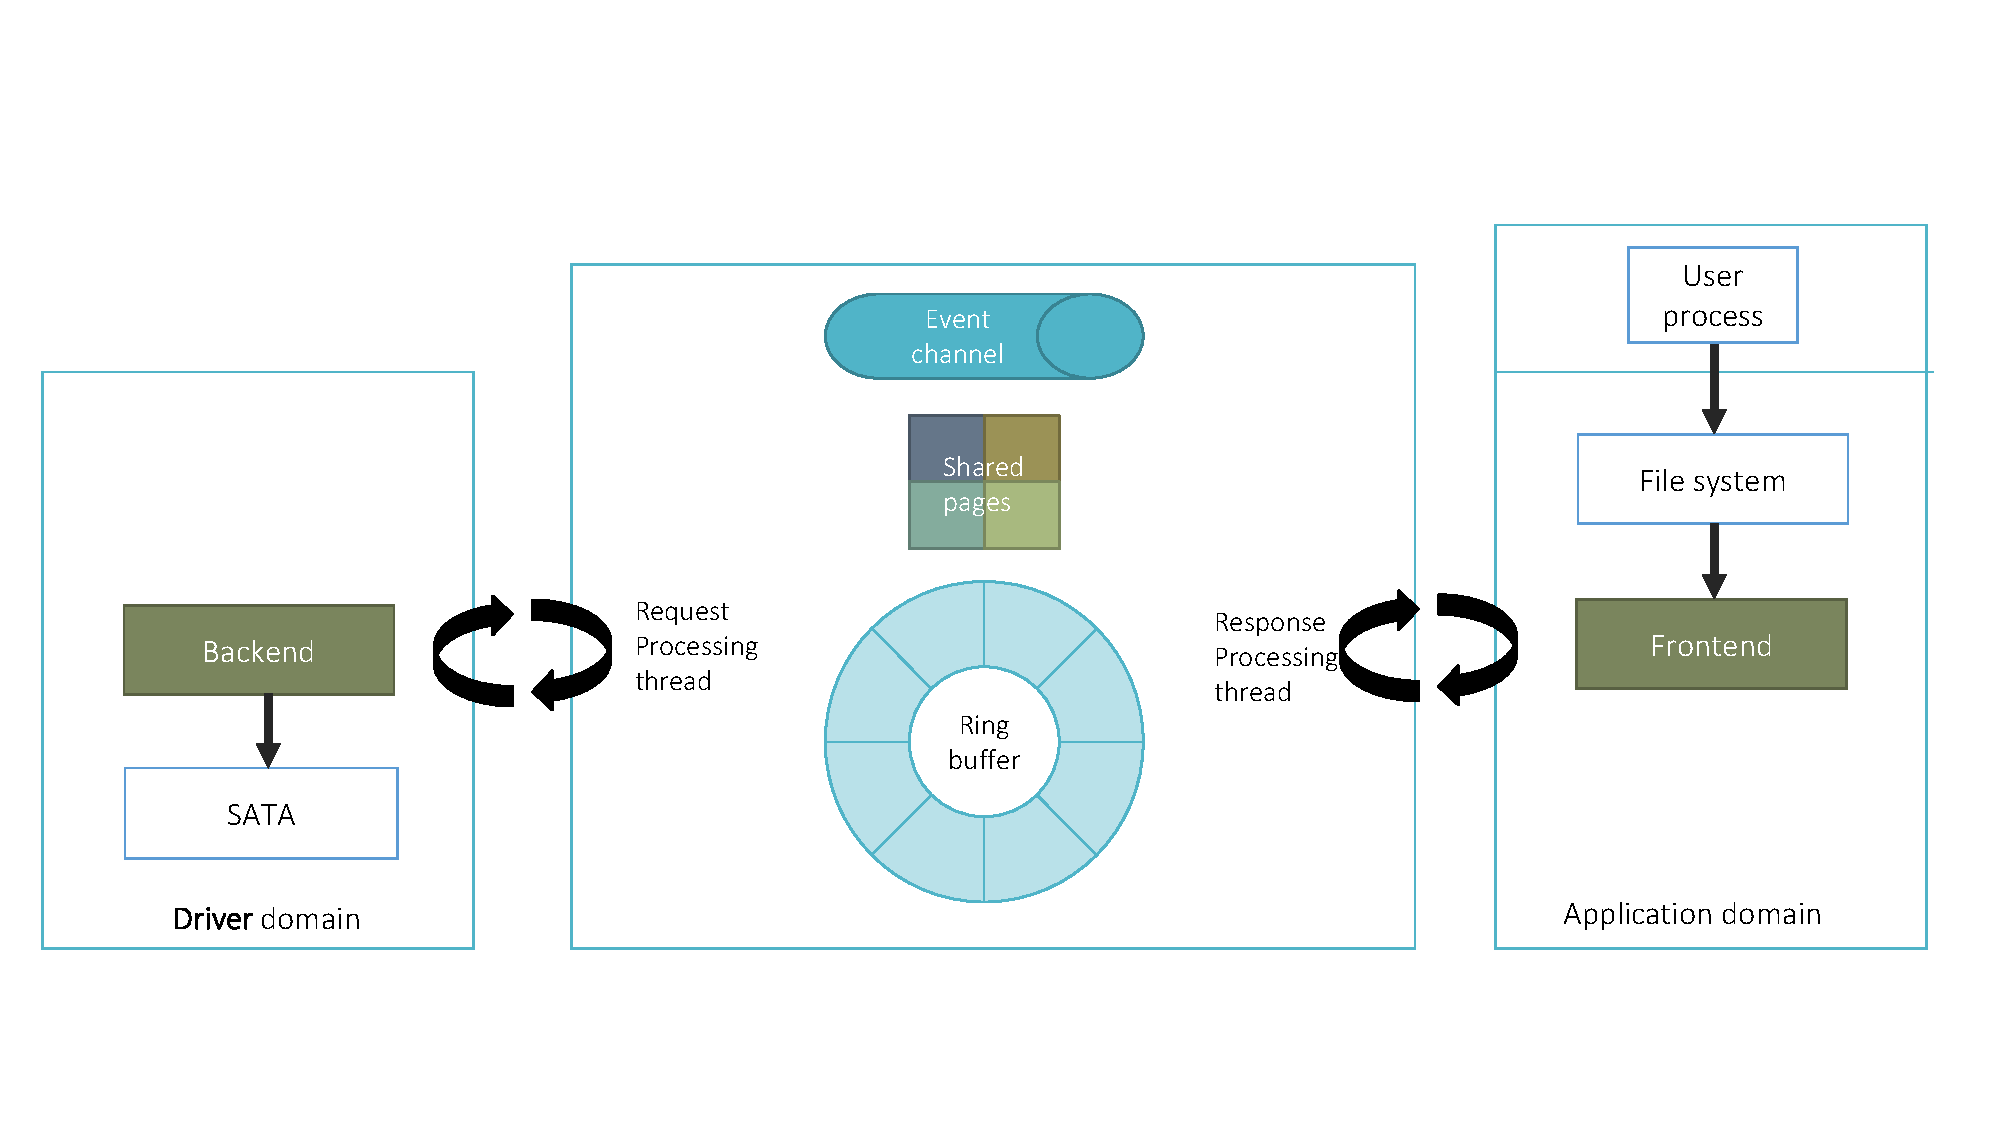
\includegraphics[scale=.5]{impl_overview}
\caption{Implementation overview}
\label{fig:Implementation overview}
\end{figure}

\subsection{Communication component}
The most important component in the IDDR system implementation is the communication component. 
\\
This section will describe the implementation details of the communication channel of the IDDR and the implementation details to improve performance of the communication channel.
\begin{enumerate}
\item In the original implementation of the IDDR, communication channel uses event channel for notifying driver domain and application domain when a request or response is available in the shared request and response queue.
\item In order to improve the performance of the IDDR system, we implement the communication channel in which the front end driver thread spins for the availability of responses, and a dedicated thread in the back end driver spins for requests. In case of unavailability of requests and responses, threads go to sleep. In this implementation event channel is used only to wake these threads up from the remote domain.
\end{enumerate}

The following subsections describe the implementation details of the communication channel with and without performance improvement measures.

\subsubsection*{Ring buffer: I/O rings}
\label{subsec:ringbuf}
In the implementation of communication channel, for both approaches, ring buffer is used as a request and response queue. Ring buffer is a shared I/O ring explained in section~\ref{subsec:io rings}. A ring buffer is divided into front ring and back ring. The front ring is used as a request queue and the back ring is used as a response queue. The front end driver recieves the request from an application, and converts the request into a format which can be understood by the back end driver. The front end device driver then checks for a free space in the request queue for a new request, and allocates the space for the new request using the function \texttt{RING\_GET\_REQUEST}. 
\\
After batching sufficient requests together, the front end device driver pushes the requests to the front ring using the function \texttt{RING\_PUSH\_REQUESTS\_AND\_CHECK\_NOTIFY}

\subsubsection*{Shared pages}
Since the ring buffer is not large enough to hold the read and write data of responses and requests, we use it only for sharing the requests and responses. In order to share an actual data we use shared pages. 

\subsubsubsection*{Grant Table} 
Grant tables are a mechanism provided by the Xen hypervisor for sharing and transferring frames between the domains. It is an interface for granting foreign access to machine frames and sharing memory between underprivileged domains provided by the Xen hypervisor. In Xen, each domain has a respective grant table data structure, which is shared with the Xen hypervisor. The grant table data structure is used by Xen to verify the access permission other domains have on the page allocated by a domain~\cite{granttable}.

\subsubsubsection*{Grant References}
Grant references are the entries in the grant table. A grant reference entry has every detail about the shared page, which removes the dependency on the real machine address of the shared page. Since there exists a fully virtualized memory, the biggest difficulty in sharing the memory correctly between domains is knowing its correct machine address. Removing the dependency with the real machine address makes it possible to share the memory between domains.\cite{Chisnall:2007:DGX:1407351, Barham:2003:XAV:945445.945462, granttable} 
\\
We use grant table so that the application domain grants the driver domain access to the the shared page, while retaining the ownership. The front end driver grants memory access to the back end driver, so that back end driver may read or write data into the shared memory as requested.
\\
The steps we implement are:
\begin{enumerate}
\item The application domain creates a grant access reference, and shares the reference id (ref) to the block device driver domain by enqueueing a request in the request queue (front I/O ring) .
\item The block device driver domain reads the request and the reference id, and uses the reference to map the foreign access granted frame.
\item The block device driver domain performs the memory access.
\item The block device driver domain unmaps the granted frame.
\item The application domain removes its grant.
\end{enumerate}

Implementation details of the above steps is explained below: 
\begin{enumerate}
\item To grant a foreign domain access, front end domain first claims a grant reference entry in the grant table using function \texttt{gnttab\_claim\_grant\_reference}, and after that grants the access to foreign domain using function \texttt{gnttab\_grant\_foreign\_access\_ref}.

\item Back end driver maps foreign frames using \texttt{gnttab\_set\_map\_op} and flags \texttt{GNTMAP\_host\_map}.

\item Back end driver unmaps the foreign frames using function \texttt{gnttab\_set\_unmap\_op} and \texttt{gnttab\_unmap\_refs}
\item Front end driver removes foreign access to the frames using function \texttt{gnttab\_end\_foreign\_access}. \texttt{gnttab\_end\_foreign\_access} does not revoke access; it only prevents further mappings. Since \texttt{gnttab\_end\_foreign\_access} does not revoke access it is used after the block device driver has unmapped the frame\cite{Chisnall:2007:DGX:1407351, Barham:2003:XAV:945445.945462}.
\end{enumerate}

\subsubsection*{Event Channel}
Event channel is a mechanism provided by xen hypervisor for event notification. Basic implementation of the IDDR communication channel uses event channel to send notifications between domains that request and response is available in the request and response queue.

\subsubsubsection*{Event channel : Hypercall interface}

\texttt{EVTCHNOP\_alloc\_unbound} is a hypercall to allocate a new event channel port. Allocated event channel port can be connected by remote domain if,
\begin{enumerate}
\item Specied domain exist
\item A free port exist in the specified domain.
\end{enumerate}
Less privileged domains can allocate only their own ports, privileged domains can also allocate ports in other domains\cite{Chisnall:2007:DGX:1407351, Barham:2003:XAV:945445.945462}. 
\texttt{bind\_evtchn\_to\_irqhandler} is used for assigning an interrupt handler for a notification.
In driver domain implementation, back end driver allocates an event channel while initializing, and assigns an interrupt handler. 

\subsubsubsection*{Event channel: Other interfaces}

\texttt{bind\_interdomain\_evtchn\_to\_irqhandler} is used for connecting to existing event channel as well as assigning an interrupt handler for handling a notification. In driver domain implementation back end driver allocates the event channel, and binds the interrupt handler to allocated event channel using \texttt{bind\_interdomain\_evtchn\_to\_irqhandler}.
\\
In driver domain implementation, front end driver connects to the event channel allocated by backend, using interface \texttt{bind\_interdomain\_evtchn\_to\_irqhandler}.

%However, in the implementation to improve the performance of the communication channel and hence the system we spin threads to share request and responses between domains and event channel is used only to wake up the both threads.

\subsection{Application domain}
Application domain is the domain running user applications. In the monolithic Linux kernel, usually an user process sends the read write request to file system, which sends the read and write request to the block device driver. The block device driver serves the request and send back a response to the file system, which further sends the response to the user process. 
\\ 
In Xen driver domain implementation block device runs separately in a driver domain. When user process sends a request to the file system, the file system needs to forward the request to storage domain. Like explained in the section~\ref{subsec:frontend}, in the implementation of xen driver domain, a piece of code is introduced which forwards the request to the domU running device drivers. 

\subsubsection*{Front end driver}

The piece of code, which forwards the request to the domU running device driver is called as a Front end driver. The core responsibility of the front end driver is:
\begin{enumerate}
\item To provide an interface which appears as a block device to upper layer in the stack.
\item Accept a request from the upper layer.
\item Create a new request which can be understood by storage domain.
\item Enqueue new request into request queue.
\end{enumerate}

Implementation details of front end driver is split into 4 stages. 
\begin{enumerate}
\item Initialization
\item Create request
\item Enqueue request 
\item Dequeue response
\end{enumerate}

\subsubsubsection*{Initialization}
During the initialization process the front end driver creates an interface for all the block devices. The interface for each block driver is associated with a queue. Read and write requests issued on the interface gets enqued in the queue. After creating the interface for all block devices, front end driver creates a kernel thread \texttt{read\_response\_thread}
\\
The core functionality of the \texttt{read\_response\_thread} is to dequeue the responses available in the ring buffer. However, there might be a case when no request is available in the ring buffer, but the request is expected to be present in the future. In such cases, \texttt{read\_response\_thread} thread spins for the responses. The \texttt{read\_response\_thread} thread goes into a sleep state after spinning for some time-threshold. 
\\
Obviously, a thread shouldn't sleep unless it is assured that somebody else, somewhere, will wake it up. The code doing the waking up job must also be able to identify the thread to be able to do its job. We use a data structure called a wait queue to find the sleeping thread. A wait queue is a list of threads, all waiting for a specific event\cite{galvin, Bovet:2005:ULK:1077084}.
\\
In Linux kernel like all other lists, a wait queue is managed by a wait queue head, of a data type \texttt{wait\_queue\_head\_t}, and is defined in \texttt{$<Linux/wait.h>$}. A wait queue head is defined and initialized statically as follows:
\texttt{DECLARE\_WAIT\_QUEUE\_HEAD(name);}
and dynamicly as follows:
\texttt{wait\_queue\_head\_t my\_queue;}
\texttt{init\_waitqueue\_head(\&my\_queue);}

\subsubsubsection*{Create request}
Front end driver dequeues the request submitted to the driver interface by a user process or the file system, and then converts the request into a request of structure type \texttt{idd\_request\_t}. The structure is as below:

\begin{verbatim}
struct idd_request {
  int data_direction; 
  uint8_t nr_segments;
  uint64_t sector_number;
  struct idd_request_segment {
      grant_ref_t gref;
      uint8_t first_sect, last_sect;
  }seg[IDD_MAX_SEGMENTS_PER_REQUEST];
  uint64_t seq_no;
}__attribute__((__packed__));
\end{verbatim}

Member of the structure are explained below.
\texttt{data\_direction} : Flag to tag if request is read or write.
\texttt{nr\_segments} : Number of \texttt{idd\_request\_segment}s.
\texttt{gref} : Grant reference\/ grant table entry.
\texttt{first\_sect} and \texttt{last\_sect} : first and last sector in frame to transfer.
\texttt{seq\_no} : To track if any request and response is lost.

\subsubsubsection*{Enqueue request}

Like explained in section~\ref{subsec:ringbuf}, \texttt{RING\_PUSH\_REQUESTS\_AND\_CHECK\_NOTIFY} is used for flushing request to the ring buffer, we use the same API to enqueue the request to the request queue. However, if the \texttt{read\_request\_thread} running in back end driver which accepts the requests is sleeping, then waking up the \texttt{read\_request\_thread} is more important task of front end driver. Wake up signal is sent to back end driver using an event channel. Before sending the notification, we check the state of the thread. Status of the thread is saved in the shared memory. We use the atomic variables to save the state of threads to avoid race conditions. 

\subsubsubsection*{Dequeue response}
Response is dequeued from the ring buffer by the \texttt{read\_response\_thread}. To dequeue the response from response queue, we use the ring buffer API \texttt{RING\_GET\_RESPONSE}. However, the important part in this stage it managing the \texttt{read\_response\_thread} thread. 
\\
When the response is not available \texttt{read\_response\_thread} spins for some time, and then goes to sleep. When the response is made available by the backend then depending upon the state of the thread, event channel interrupt is sent by the backend. If \texttt{read\_response\_thread} is in sleeping state then the backend driver will send an interrupt and the front end driver will wake up the thread, otherwise, no action is taken as thread is already spinning for the response.
\\
In interrupt handler shared atomic variable status is read by the front end driver and depending upon state action is taken. \texttt{read\_response\_thread} sleeps on the wait queue, waiting for a flag denoting availability of the response to be set. Once the response is available in the response queue, it is read using  ring buffer API \texttt{RING\_GET\_RESPONSE}.
\\
We also maintain an shadow table of all requests submitted to the back end driver. The requests are read from the shadow table and are ended upon successfully reading the respective response. The request is ended by using a function \texttt{\_\_blk\_end\_request\_all}
\\
Upon reading the responses, thread spins again for more responses and after reaching the threshold goes to sleep. We mark the state of the thread as \texttt{SLEEPING} and then check for the request queue to avoid race condition. If a request is present in the request queue then the request is served while state of the thread is still \texttt{SLEEPING}.

\subsection{Driver domain}

Driver domain is the domU running a device driver. In our implementation, driver domain runs block device driver. Usually in monolithic Linux kernel an user process sends the read write request to a file system, which sends the read and write request to block device driver. Block device driver serves the request and responses back to file system, which further sends response to user process.
\\  
However, in driver domain implementation, block device runs separately in a driver domain. Like explained in a section~\ref{subsec:backend}, a piece of code called as a back end driver runs in a driver domain which accepts a request from application domain and forward the request to the device driver. Upon receiving the response from the device driver, back end driver sends back the response, and notifies the application domain.

\subsubsection*{Back end driver}

Back end driver is a kernel module and component of IDDR which runs in the driver domain. The core responsibility of back end end driver is :
\begin{enumerate}
\item Dequeue request from request queue.
\item Convert to BIO request which can be understood by block device driver.
\item Accept response from block device driver.
\item Enqueue response into response queue.
\end{enumerate}
Implementation details of back end driver can be split into 5 stages. 
\begin{enumerate}
\item Initialization
\item Dequeue request
\item Create BIO. 
\item Make response.
\item Enqueue response
\end{enumerate}

\subsubsubsection*{Initialization}
During initialization process Back end driver creates a kernel thread \texttt{read\_request\_thread}. The core functionality of the \texttt{read\_request\_thread} is to dequeue the requests available in the request queue. If request is not available in the request queue then thread waits on a wait queue. Similar to front end, back end driver initializes wait queue in initiazation process. 

\subsubsubsection*{Dequeue request}
Request is dequeued from the request queue by the \texttt{read\_request\_thread}. To dequeue a request, we use the ring buffer API \texttt{RING\_GET\_RESPONSE}. When the request queue is empty, \texttt{read\_request\_thread} spins for some time to checks if new requests are queued, after reaching threshold it goes to sleep. When the request is enqueued by front end driver then depending upon the state of the \texttt{read\_request\_thread}, an event channel interrupt is sent by the front end driver. If \texttt{read\_request\_thread} is in a sleeping state then front end driver will send an interrupt. In intrupt handler, back end driver will wake up the \texttt{read\_request\_thread}. If \texttt{read\_request\_thread} is already running then no action is taken. In interrupt handler, status is read from shared atomic variable by the back end driver.
\\
\texttt{read\_request\_thread} sleeps on a wait queue waiting for a flag to be set. The flag denotes the avilability of the request in the request queue. The request is read from the request queue using ring buffer API \texttt{RING\_GET\_REQUESTS}.
\\
After reading the requests, \texttt{read\_request\_thread} thread spins again for more requests. If a threshold limit is reached then the \texttt{read\_request\_thread} thread goes to sleep. We mark the state of the thread as \texttt{SLEEPING} and then check for the request queue one more time to avoid a race condition. If request is present in request queue then that request is served while state of the thread is still \texttt{SLEEPING}.

\subsubsubsection*{Create BIO}
\label{subsec:createbio}
Whenever the request thread receives a request to serve, the request thread creates the \texttt{bio} request for the corresponding request. \texttt{bio} structure is a basic container for block I/O within a kernel. \texttt{bio} structure is defined in \texttt{$<Linux/blk_types.h>$}. \texttt{bio} structure represents active block I/O operations as a list of segments, and a segment is a chunk of buffers. The \texttt{bio} structure provides the capability for the kernel to perform block I/O operations of even a single buffer from multiple locations in memory. Vector I/O such as this is called scatter-gather I/O.
\\
% Following is the struct bio:
% \begin{verbatim}
% struct bio {
%   sector_t    bi_sector;  /* device address in 512 byte sectors */
%   struct bio    *bi_next; /* request queue link */
%   struct block_device *bi_bdev; /* associated block device */
%   unsigned long   bi_flags; /* status, command, etc */
%   unsigned long   bi_rw;    /* bottom bits READ/WRITE, top bits priority */
%   unsigned short  bi_vcnt;  /* how many bio_vec's */
%   unsigned short  bi_idx;   /* current index into bvl_vec */
%   unsigned int    bi_phys_segments; /* Number of segments in this BIO after physical address coalescing is performed. */
%   unsigned int    bi_size;  /* residual I/O count */
%   unsigned int    bi_seg_front_size;
%   unsigned int    bi_seg_back_size;
%   unsigned int    bi_max_vecs;  /* max bvl_vecs we can hold */
%   atomic_t    bi_cnt;   /* pin count */
%   struct bio_vec    *bi_io_vec; /* the actual vec list */
%   bio_end_io_t    *bi_end_io;  void      *bi_private;
%   bio_destructor_t  *bi_destructor; /* destructor */
%   struct bio_vec    bi_inline_vecs[0];
% };
% \end{verbatim}
A request queued into the request queue by the front end driver is in format which is understood by back end driver, but we cannot forward the same request to block device. We convert the dequeued request into \texttt{bio} request, so that the block device understands the request. In order to make the \texttt{bio} request, we need the associated block device structure \texttt{struct block\_device}. We get associated block device structure using function \texttt{blkdev\_get\_by\_path}. 
\\
Pages from shared memory are mapped and inserted into the \texttt{bio} structure using function \texttt{bio\_add\_page}. And other variables are copied into the \texttt{bio} structure from the dequeued request. At the end, the newly created \texttt{bio} request is sent to the lower layer for execution with \texttt{submit\_bio}. Once bio request is completed, function pointed by a function pointer \texttt{bi\_end\_io} gets called.

\subsubsubsection*{Make response and Enqueue}
Irrespective of the success or failure of the execution of \texttt{bio} request, the back end driver makes a response, which could be understood by the frontend. Like explained in subsection~\ref{subsec:createbio}, \texttt{bi\_end\_io} function pointer is a pointer to a callback function. Once bio request is completed, function pointed by \texttt{bi\_end\_io} gets called. We create a new response in this callback function.
\\
In this callback function we complete the \texttt{bio} request with function \texttt{bio\_put}. After that the result gets copied into a newly allocated response structure. The response is enqueued to response queue using \texttt{RING\_GET\_RESPONSE} and \texttt{RING\_PUSH\_RESPONSES\_AND\_CHECK\_NOTIFY}. Once the response is enqueued, depending upon the status of the remote thread-\texttt{read\_response\_thread}, a interrupt signal is sent to the application domain.

% \bibliography{references}
\ifbool{toShowBibliography}{\bibliography{references}}{}